\documentclass[
  12pt, % Fontsize
  a4paper, % papersize
  oneside, % For twosided documents
  openany, 
  numbers=noenddot, % No final dots in Sectionnumbers, e.g 1.2 instead of 1.2.
  BCOR=5mm, % Correction length for lost space from binding
  parskip=half*, %No indent but spacing between paragraphs
  thesis, % type of document
]{bfhbook}


% Test Template for bfhbook.cls
\usepackage[T1]{fontenc}
% Coding 
\usepackage[utf8]{inputenc}
% Language setting
\usepackage[german]{babel}
\usepackage[export]{adjustbox}

% \usepackage{fonttable}
% Hyperref
\usepackage[                
  pdftex,                  % for PDF
  colorlinks=true,         % colored links
  linkcolor=black,         % color for links
  citecolor=black,         % color for references
  urlcolor=black,          % color for url 
  bookmarks=true
]{hyperref}              

\usepackage{booktabs} % For nicer tables
\usepackage{threeparttable} % Table-Captions having the same width than the table
\usepackage[singlelinecheck=off]{caption}
\usepackage{siunitx} % Scientific Units and number setting

\definecolor{codegreen}{rgb}{0,0.6,0}
\definecolor{codegray}{rgb}{0.5,0.5,0.5}
\definecolor{codepurple}{rgb}{0.58,0,0.82}
\definecolor{backcolour}{rgb}{0.95,0.95,0.95}

\usepackage{listings} % For Program-Code
\lstdefinestyle{mystyle}{
    backgroundcolor=\color{backcolour},   
    commentstyle=\color{codegreen},
    keywordstyle=\color{magenta},
    numberstyle=\tiny\color{codegray},
    stringstyle=\color{codepurple},
    basicstyle=\ttfamily\footnotesize,
    breakatwhitespace=false,         
    breaklines=true,                 
    captionpos=b,                    
    keepspaces=true,                 
    numbers=left,                    
    numbersep=5pt,                  
    showspaces=false,                
    showstringspaces=false,
    showtabs=false,                  
    tabsize=2
}
 
\lstset{style=mystyle}

\usepackage{enumitem}
\setlist[description]{style=nextline}

\usepackage{caption}
\captionsetup[figure]{font=footnotesize, labelfont=small}
\newcommand{\source}[1]{\caption*{Quelle: {#1}} }

\usepackage{xcolor}

\usepackage[export]{adjustbox}
\usepackage[document]{ragged2e} % left-alignment for text

\usepackage[acronym]{glossaries}

\definecolor{foldercolor}{RGB}{124,166,198}

\usepackage[style=apa]{biblatex}
\addbibresource{references.bib}

\ExecuteBibliographyOptions{labelnumber}
\DeclareFieldFormat{labelnumberwidth}{\mkbibbrackets{#1}}

% bib environment for numeric citations (@online) from numeric.bbx
\defbibenvironment{onlinebib}
  {\list
     {\printtext[labelnumberwidth]{%
        \printfield{labelprefix}%
        \printfield{labelnumber}}}
     {\setlength{\labelwidth}{\labelnumberwidth}%
      \setlength{\leftmargin}{\labelwidth}%
      \setlength{\labelsep}{\biblabelsep}%
      \addtolength{\leftmargin}{\labelsep}%
      \setlength{\itemsep}{\bibitemsep}%
      \setlength{\parsep}{\bibparsep}}%
      \renewcommand*{\makelabel}[1]{\hss##1}}
  {\endlist}
  {\item}

% taken from numeric.cbx
\providebool{bbx:subentry}
\newbibmacro*{cite:num}{%
  \printtext[bibhyperref]{%
    \printfield{labelprefix}%
    \printfield{labelnumber}%
    \ifbool{bbx:subentry}
      {\printfield{entrysetcount}}
      {}}}

% switch citation style based on entry type
\DeclareCiteCommand{\parencite}
  {\ifentrytype{misc}{\bibopenbracket}{\bibopenparen}%
   \usebibmacro{prenote}}%
  {\usebibmacro{citeindex}%
   \ifentrytype{misc}{\usebibmacro{cite:num}}{\usebibmacro{cite}}}
  {\multicitedelim}
  {\usebibmacro{postnote}%
   \ifentrytype{misc}{\bibclosebracket}{\bibcloseparen}}

% end definition directory tree

%%%%%%%%%%%%%%%%%%%%%%%%%%%%%%%%%%%
% Settings 
%%%%%%%%%%%%%%%%%%%%%%%%%%%%%%%%
% Type?? (Lecture Notes, BSc Thesis, Master Thesis, . . .) 
% Use Variables \BSc, \Master, etc. for language support
\type{Master Thesis}
% Author(s)
\author{Marc Habegger}
% Title
\title{Explainable AI}
% Short Title, will be used in the footline
\shorttitle{MAS Data Science Master Thesis}
% Subtitle
\subtitle{Stand der Forschung und Technik}
% Titlepicture
% \titlepicture{Bilder/Titel.png}
%%

% Topic of Study
\degreeprogramme{MAS Data Science}
% Expert
\expert{Max Kleiner}
% Version
\version{1.0}
% Date
\date{\today} % Or any other possible date

% Departement
% Use Variable for language support
%\TI

% Semester
% Use Variable for language support
%\semester

% Logo(s)

% Colors
% Secondary Color for Graphics, Tables etc.
% Naming: BFH*Color*light|middle|dark, e.g. BFHGreendark, BFHBluelight, etc.
% Possible Color Values: Green, Blue, Purple, Brown 
\newcommand{\seccolor}{BFHLightGreen} 
\newcommand{\imgText}[3]{
\begin{center}
    \begin{minipage}[t]{0.6\textwidth}
    		\vspace{0pt}
		\includegraphics[width=10cm, left]{Bilder/#1}
		\caption{#2}
	\end{minipage}\hfill
    \begin{minipage}[t]{0.4\textwidth}
    		\vspace{20pt}
  		#3
    \end{minipage}
\end{center}
}

\newcommand{\fullImg}[2]{
\begin{center}
  \begin{minipage}{\linewidth}
    \centering
    \includegraphics[width=\linewidth]{Bilder/#1}
    \captionof{figure}{#2}
  \end{minipage}
\end{center}
}

\setcounter{secnumdepth}{4}
\setcounter{tocdepth}{4}

% Variablen für diese Arbeit
\newcommand{\compImgSize}{4cm}

% Glossar Einträge
\makeindex
% Generate the glossary
\makeglossaries


\newglossaryentry{MLg}
{
	name=Machine Learning,
	description={deutsch Maschinelles lernen. Ein künstliches System lernt aus Beispielen und kann diese nach Beendigung der Lernphase verallgemeinern. }
}

\newglossaryentry{AIg}
{
	name=Artificial Intelligence,
	description={deutsch Künstliche Intelligenz. Nicht scharf abzugrenzender Bereich des Machine Learning in dem versucht wird ein intelligentes Verhalten
	 analog menschlicher oder tierischer Verhaltensweisen nachzubilden. }
}

\newglossaryentry{XAI}
{
	name=Explainable Artificial Intelligence,
	description={deutsch erklärbare künstliche Inteligenz, Methodiken um Menschen die Vorhersagen durch Modelle des maschinellen Lernens zu erläutern. }
}

\newglossaryentry{DNN}
{
    name=Deep Neural Network,
    description={deutsch tiefes lernen, Bezeichnet Neuronale Netze mit vielen Zwischenschichten.}
}

\newglossaryentry{NN}                                 
{
	name=Neuronales Netz,
	description={}   
}   

\newglossaryentry{LRP}                                 
{
	name=Layer-wise Relevance Propagation,
	description={Technik zur Bestimmung der Merkmale welche am stärksten für das Endresultat verantwortlich sind.}                                   
}                          

\newglossaryentry{Black Box}                                 
{
	name=Black Box,
	description={System welches nicht im Quellcode vorhanden ist und dadurch nicht durch Analyse der Programmierung verstanden werden kann. Jegliche Rückschlüsse sind nur durch Beobachtungen möglich}                                   
}     

\newglossaryentry{DT}                                 
{
	name=Decision Tree,
	description={Entscheidungsbaum, Familie von ML Algorithmen}                                   
}     

\newglossaryentry{GC}
{
	name=Grad CAM,
	description={Gradient-weighted Class Activation Mapping, Technik welche für eine Entscheidung relevanten Bildinhalte optisch hervorhebt}  
}

\newglossaryentry{KH}
{
	name=Kluger-Hans-Effekt,
	description={``Kluger Hans'' war ein Pferd aus dem Anfang des 20. Jahrhunderts das angeblich rechnen und zählen konnte, jedoch auf  die feinen Nuancen der Mimik und Körpersprache des Fragestellers reagierte. Seitdem wird als ``Kluger-Hans-Effekt'' eine unbewusste beeinflussung des Studienobjektes bezeichnet. In Machine Learning Lösungen kann der ``Kluger-Hans-Effekt'' auftauchen wenn ein Model mit Daten traniert wird welche die Vorhersage unbewusst in eine bestimmte Richtung lenken.}  
}

\newglossaryentry{OS}
{
	name=Occlusion Sensitivity,
	description={Verfahren um die für eine Klassifikation relevanten Bildinhalte zu finden indem bestimmte Bildinhalte entfernt werden (Occlusion) und die dabei entstehende Veränderung auf die Klassifikation gemessen wird.}  
}

\newglossaryentry{GI}
{
	name=Gradients Input,
	description={}  
}

\newglossaryentry{BIAS}
{
	name=Bias,
	description={Bias, deutsch Tendenz oder Voreingenommenheit, kann in Machine Learning Modellen auftreten wenn die Trainingsdaten unausgewogen sind. Dies kann zu einer sogenannten selbsterfüllenden Prophezeiung werden indem die Resultate des Models zu neuen Trainingsdatensätzen führen welche die Tendenz noch verstärken.}  
}

\newglossaryentry{limeG}
{
	name=LIME,
	description={Local interpretable model-agnostic explanations, eine unabhängig des verwendeten Algorithmus anwendbare Erklärungstechnik für Black Box Modelle }
}

\newglossaryentry{tcavG}
{
	name=Testing with Concept Activation Vectors,
	description={Technik welche Erklärungen einer Klassifikation durch Erkennung der Bildbestandteile erzeugt. Benutzt dafür Neuronale Netze welche auf einzelnen Bestandteile trainiert werden. \parencite{Kim2017}}
}

\newglossaryentry{av}
{
	name=Activation Vector (Aktivierungsvektor),
	description={In einem Neuronalen Netzwerk erzeugt ein Neuron für jedes Bild welches Analysiert wird einen bestimmten Ausgangswert. Für mehrere Bilder bilden die jeweiligen Ausgangswerte des Neurons den sogenannten Aktivierungsvektor.}
}

\newglossaryentry{svccaG}
{
	name=SVCCA,
     description={Singular Vector Canonical Correlation Analysis, ein Verfahren welches Aktivierungs Vektoren eines Neuronalen Netzes vergleicht. Der Vergleich kann entweder zwischen den Layern eines Netzes oder zwischen unterschiedlichen Netzen durchgeführt werden. \parencite{Raghu2017}}
}

\newglossaryentry{binClassificator}
{
	name=Binärer Klassifikator,
     description={Ein binärer Klassifikator ist eine Sonderform eines Klassifikators welche nur eine Klasse kennt. Häufig sind das ja/nein Fragen zum Beispiel ``ist auf diesem Bild ein Tumor erkennbar?''.}
}

\newacronym{ML}{ML}{Machine Learning}

\newacronym{AI}{AI}{Artificial Intelligence}

\newacronym{cnn}{CNN}{Convolutional Neural Network}

\newacronym{dnn}{DNN}{Deep Neural Network}

\newacronym{lrp}{LRP}{Layer-wise Relevance Propagation}

\newacronym{lime}{LIME}{Local interpretable model-agnostic explanations}

\newacronym{tcav}{TCAV}{Testing with Concept Activation Vectors}

\newacronym{svcca}{SVCCA}{Singular Vector Canonical Correlation Analysis}

\newacronym{xai}{XAI}{Explainable artificial intelligence}

\newacronym{glm}{GLM}{Generalized Linear Models}

\newacronym{gam}{GAM}{Generalized Additive Models}

\newacronym{lfr}{LFR}{Learned fair representations}

\newacronym{m-gbm}{M-GBM}{Monotonic gradient boosting}

\newacronym{pate}{PATE}{Private aggregation of teacher ensembles}

\newacronym{sbrl}{SBRL}{Scalable Bayesian rule list}

\newacronym{slim}{SLIM}{Supersparse linear integer models}

\newacronym{dek}{DEK}{Datenethikkommission}

\newacronym{gradcam}{Grad CAM}{Gradient-weighted Class Activation Mapping}

\newacronym{aip}{AIP}{Adversarial Image Perturbations}


\begin{document}
                         
\maketitle
%**************************************************************************
%\frontmatter % preliminary parts

\tableofcontents
\sloppy
%%%%%%%%%%%%%%%%%%%%%%%%
% Introduction
%**************************************************************************
\mainmatter % The main part
%**************************************************************************
%\part{Part One}

\chapter{Einleitung}
Computer Programme bestehen in der Regel aus tausenden bis Millionen Zeilen von Anweisungen welche für die verschiedenen Aspekte eines Programmes zuständig sind. Einige der Programmroutinen stellen die grafische Benutzeroberfläche dar während andere sich um das Speichern und laden von Dateien kümmern. Andere wiederum definieren Regeln nach denen Daten verarbeitet und analysiert werden. Solche Regeln werden von Fachspezialisten definiert und durch Software-Entwickler umgesetzt. Mit einem derartigen Vorgehen konnten viele alltägliche Probleme gelöst werden und Software ist inzwischen in der Wirtschaft wie im privaten Umfeld allgegenwärtig geworden. 
\paragraph*{}
Die Ausformulierung solcher Regeln nach denen sich Software verhalten soll ist aber ein aufwendiger und fehlerträchtiger Prozess und gewisse Gebiete waren durch die Komplexität der Aufgabenstellung nur rudimentär in Regeln zu fassen. Solche Gebiete sind unter anderem Bilderkennung, Text- oder Sprachverständnis, Gebiete in denen Menschen und Tiere bedeutend bessere Fähigkeiten zeigen als Computer Programme. 
\paragraph*{}
Während programmierte Regeln in Computer Programmen sofort zur Verfügung stehen müssen Menschen und Tiere ihre Fähigkeiten oftmals über längere Zeit trainieren und üben bis die gewünschten Fähigkeiten in genügender Qualität vorhanden sind. Durch solche biologische Prozesse als Vorbild wurde die Disziplin \gls{ML} entwickelt, welche auch Computer in die Lage versetzen soll, bislang nur bei Mensch und Tier gefundene Fähigkeiten, zu erlangen.
\gls{ML} wird seit den 1960er Jahren angewendet, allerdings waren die erzielten Resultate lange Zeit für viele Anwendungen ungenügend. Durch die Verfügbarkeit von grossen Datenmengen (Big Data, Cloud) und der gesteigerten Rechenleistung der Rechner wurden nach der Jahrtausendwende so gute Fortschritte erzielt dass immer mehr Anwendungsmöglichkeiten für \gls{ML} Lösungen gefunden wurden. 

\fullImg{ML-Timeline.png}{Entwicklung des Machine Learning als Zeitachse}

Durch die Anwendung von Versuch und Irrtum bei kontinuierlicher Optimierung der internen Regeln erlangten \gls{ML} Systeme bislang unerreichbare Stärken in vorher problematischen Gebieten. Allerdings ist der Preis dafür oftmals der, dass die automatisch erstellten Regeln für Menschen unverständlich und nicht nachvollziehbar sind.
Für viele Dienste im Internet (Bildersammlungen, Empfehlungssysteme) werden in der Regel keine oder nur geringe Anforderungen an ein verständliches Modell gestellt. Aber es gibt einige Bereiche in denen besondere Ansprüche an die Nachvollziehbarkeit von Entscheidungen bestehen.

 Exemplarisch werden hier einige dieser Gebiete aufgeführt:

\begin{description}
  \item[Medizin] \gls{ML} Anwendungen für die Krebserkennung bieten grosses Potenzial. Insbesondere die ermüdenden Aufgabe auf Röntgen- oder MRT-Bildern Spuren eines Tumors zu erkennen könnten durch \gls{ML} abgelöst werden. Allerdings sind die Zulassungskriterien für solche Lösungen noch nicht definiert.
  \item[Justiz] Predictive Policing versucht mittels statistischer und \gls{ML} Verfahren Orte oder Personengruppen zu erkennen welche  Schauplatz oder Täter/Opfer eines Verbrechens werden könnten.
  \item[Selbstfahrende Fahrzeuge] Obwohl Selbstfahrende Fahrzeuge seit Jahren von allen grossen Fahrzeugherstellern entwickelt werden sind immer noch viele Fragen bezüglich der Haftung und Zulassung offen.
\end{description}

Aufgrund des Mangels an Techniken um fortgeschrittene \gls{ML} System zu Verstehen, entstand deshalb ein neues Forschungsgebiet \acrfull{xai} welches sich zum Ziel gesetzt hat Methoden und Werkzeuge zu entwickeln um \gls{ML} Modelle zu analysieren.

\chapter{Was bedeutet Erklärbarkeit?}
\gls{ML} erzeugt Resultate welche je nach Anwendungsfall eine Entscheidung für Klasse (Pferd, Schaf, Auto), eine Zuordnung zu einer Gruppe (Premium-Kunde, Gelegenheitskäufer etc.) oder es wird ein numerischer Wert generiert (15 Grad Celsius am 3. April). 
Da sowohl die Erzeugung des Models als auch die Berechnung des Resultates automatisch erfolgt können die Schritte auf dem Weg zu dem Resultat nicht direkt nachvollzogen werden.

\begin{figure}[ht]
\centering

\includegraphics[width=\textwidth]{Bilder/Explanation-Flow.png}
\caption{Ablauf einer erklärbaren Machine Learning Anwendung}
\end{figure}

Eine \Gls{ML} Lösung beginnt mit der Beobachtung von realen Ereignissen in der Welt. Dies können die Anzahl Blätter und deren Länge einer Pflanzungsgattung oder auch Häuserpreise in Brooklyn sein. Diese Beobachtungen werden gesammelt und bilden die Daten Grundlage mit deren ein Model erzeugt werden kann. Aus diesem Model kann eine Erklärung erzeugt werden die ein Mensch verwenden kann um das Resultat zu erklären.
\section{Unterschiedliche Ziele}
Eine Anwendung welche \Gls{ML} einsetzt kann in mehrere Bereiche unterteilt werden.  Durch diese Aufteilung in verschiedene  Komponenten ergeben sich unterschiedliche Anforderungen an die Erklärbarkeit: \parencite{XAI2018}

\begin{description}
\item[Daten]
Aus der Sicht der Daten interessiert vor allem welcher Teil der Daten für das Ergebnis die Grösste Relevanz hat. Basierend auf dieser Erkenntnis kann das Datenset gezielt erweitert werden oder auch reduziert so dass ein ausgeglichenes Verhältnis erzeugt wird.

\item[Modell]
Kann man aus dem Modell Muster für eine bestimmte Kategorie ableiten? Dies kann helfen Fehlklassifizierungen von zusätzlichen Daten zu verhindern in dem überprüft wird ob das Modell die richtigen Features berücksichtigt.

\item[Vorhersage]
Erklärung weshalb ein bestimmtes Muster in den Daten zu der beobachteten Klassifizierung geführt hat. Dies ist insbesondere für Anwender/Kunden einer ML Lösung um a) das Verständnis für die Maschinelle Entscheidung zu erhöhen oder b) eine gesetzlich Vorgeschriebene Anfechtbarkeit der Entscheidung zu ermöglichen.
\end{description}

Ebenso gibt es bei den Interessengruppe unterschiedliche Anforderungen an die Erklärbarkeit einer ML Anwendung. Nach \parencite{Ras2018} werden dabei folgende Gruppierungen unterschieden:
\begin{description}
  \item[Experten]
  Diese Gruppe kann weiter unterteilt werden in
  	\begin{description}
  		\item[Forscher] Entwickelt neue Methoden und Algorithmen für das ML, verbessert bestehende Algorithmen
  		\item[Entwickler] Setzt bestehende Methodiken und Algorithmen ein um eine konkrete Aufgabenstellung zu lösen
	\end{description}
  \item[Benutzer]
  Auch bei den Benutzern gibt es verschiedene Ausprägungen
  	\begin{description}
  		\item[Eigentümer]
  		\item[Anwender]
  		\item[Person deren Daten verwendete wird]
  		\item[Anspruchsgruppe (Stakeholder)]
	\end{description}
\end{description}
Die Anforderungen an ein erklärbares Modell unterscheiden sich so stark je nach betrachtetet Komponente und der Anwendergruppe. Daraus ergibt sich dass verschiedene Techniken benötigt werden um AI Lösungen generell erklärbar zu machen.

\section{Herausforderungen durch Datenschutz}
Der jüngste Bericht der \acrfull{dek} der Deutschen Regierung \parencite{datenEthik} geht in Kapitel 3. konkret auf  \Gls{ML} Anwendungen ein.
\break
Unter dem Begriff ``algorithmische Systeme'' werden anhand von drei Kategorien Anforderungen gestellt.
\break
 Die von der  \acrshort{dek} definierten Bereiche sind:
 
 \begin{enumerate}
   \item  algorithmenbasierte Entscheidungen sind menschliche Entscheidungen, die sich auf algorithmisch berechnete (Teil-)Informationen stützen
   \item algorithmengetriebene Entscheidungen sind menschliche Entscheidungen, die durch die Ergebnisse algorithmischer Systeme in einer Weise geprägt werden, dass der tatsächliche Entscheidungsspielraum und damit die Selbstbestimmung des Menschen eingeschränkt werden
   \item  algorithmendeterminierte Entscheidungen führen automatisiert zu Konsequenzen, so dass im Einzelfall keine menschliche Entscheidung mehr vorgesehen ist
\end{enumerate}

Daraus ergeben sich für die \acrlong{dek} für einen verantwortungsvollen Umgang mit ``algorithmischen Systemen'' folgende Grundsätze an denen man sich orientieren sollte:

\begin{itemize}
	\item Menschenzentriertes Design
	\item Vereinbarkeit mit gesellschaftlichen Grundwerten
	\item Nachhaltigkeit
	\item Qualität und Leistungsfähigkeit
	\item Robustheit und Sicherheit
	\item Minimierung von Verzerrungen und Diskriminierung
	\item Transparenz, Erklärbarkeit und Nachvollziehbarkeit
	\item Klare Rechenschaftsstrukturen
\end{itemize}

\acrlong{xai} kommt vor allem in den Bereichen ``Minimierung von Verzerrungen und Diskriminierung'' und ``Transparenz, Erklärbarkeit und Nachvollziehbarkeit'' zum tragen, kann aber auch bei ``Robustheit und Sicherheit'' und ``Qualität und Leistungsfähigkeit'' helfen.

\section{Diskriminierung}

\section{Bessere Anwendungen durch Einblick in die Funktionsweise}

\section{Weniger Angriffsflächen}

\section{Haftungsfragen}

\chapter{Anwendung von XAI auf Modelle}
Nach \parencite{Oh2019} hat Art des Modells von grossem Einfluss auf die Möglichkeiten der Erklärbarkeit. Generell wird unterschieden zwischen
\begin{description}
\item[Whitebox Modelle] sind unter der Kontrolle desjenigen welcher eine erklärende Analyse durchführt, sowohl die Daten wie der Aufbau des Modelles sind bekannt
\item[Blackbox Modelle] sind von unbekannter Struktur, der Anwender bekommt von einem gegebenen Input ein Resultat ohne den Ablauf der Entscheidungsfindung beobachten zu können
\end{description}

Aus der Vielzahl von Werkzeugen welche existieren um \acrfull{ML} Modelle zu analysieren gilt es die für den jeweiligen Use Case relevanten Werkzeuge anzuwenden.
TODO: Übersicht der Techniken und Anwendungsbereiche wie in der Grafik

\section{Anwendungsfälle}
\subsection{Exploration}
\begin{itemize}
	\item Biplot
	\item Darstellung der Korrelation (Correlation graph)
	\item Korrelationsmatrix
	\item Heatmap
	\item Parallele Koordinatendarstellung (Parallel coordinates plot)
	\item Projektion MDS, 1-SNE, UMAP
	\item Radar Plot
	\item Scatter Plot
	\item Univariate Statistiken: Häufigkeits-Verteilung, Histogram, Pivot-Tabelle
\end{itemize}
\subsection{Feature Engineering}
\subsection{Ein interpretierbares Model erstellen}
\begin{itemize}
	\item Entscheidungsbaum
	\item \acrfull{gam}
	\item \acrfull{glm}
	\item \acrfull{lfr}
	\item \acrfull{m-gbm}
	\item \acrfull{pate}	
	\item \acrfull{sbrl}
	\item \acrfull{slim}
\end{itemize}
\subsection{Modelle interpretieren}
Neben vielen Methoden welche nur für bestimmte Klassen von Verfahren anwendbar sind, gibt es einige die Allgemein anwendbar sind.

\begin{itemize}
	\item[LIME] \ref{lime}
\end{itemize}

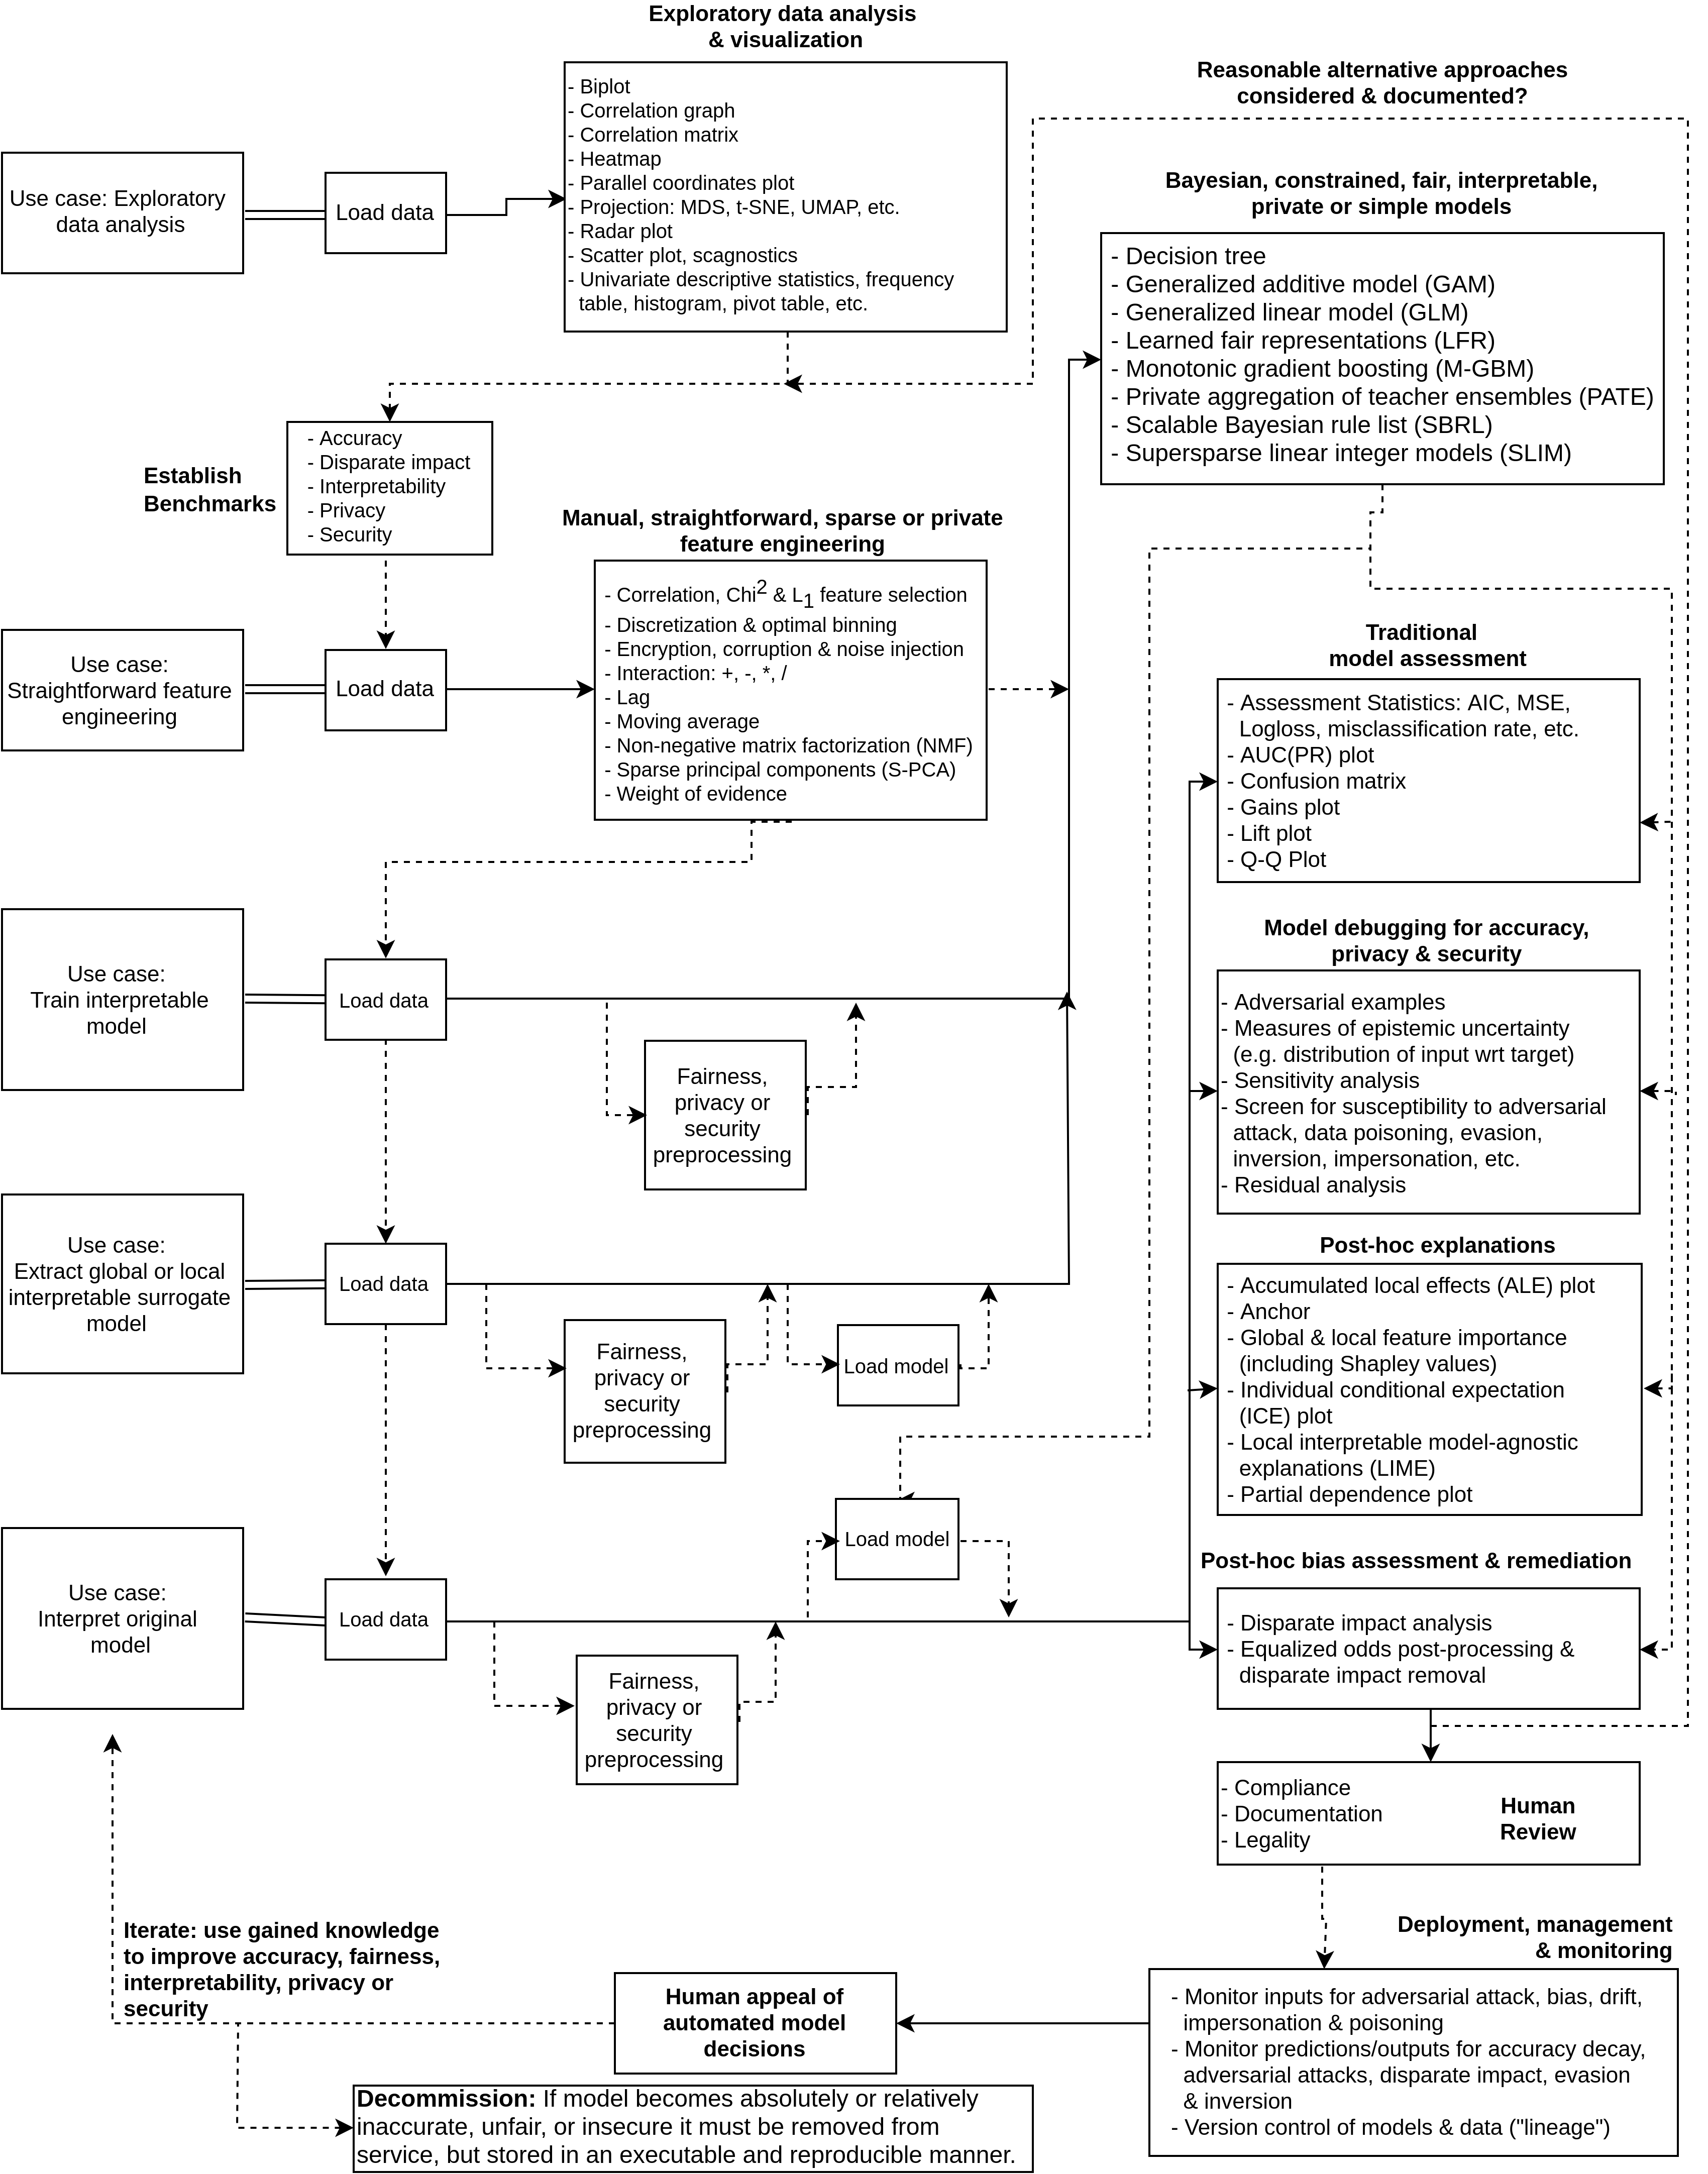
\includegraphics[width=\textwidth]{Bilder/blueprint.png}
\captionof{figure}{Quelle: https://github.com/h2oai/mli-resources}

\section{Grundsätzlich erklärbare Algorithmen}
\subsection{Lineare Regression}
Lineare Regression ist seit langer Zeit ein nützliches Werkzeug für Statistiker und Informatiker. Die Zusammenhänge zwischen dem Berechneten Ergebnis und den Eingangsvariablen können einfach nachvollzogen werden. Lineare Regression ist weit verbreitet, auch in nicht Informatik nahen Gebieten wie Medizin oder Soziologie. Ein Nachteil dieser Methode ist jedoch kleinere Leistungsfähigkeit in Bezug auf die Vorhersagequalität so dass heutzutage oftmals auf leistungsfähigere, jedoch schlechter verständliche, Algorithmen zurückgegriffen wird. Insbesondere im Gebiet der Klassifikation zeigt die Lineare Regression Schwächen.

\begin{center}
\begin{minipage}[t]{0.45\linewidth}
\vspace{0pt}
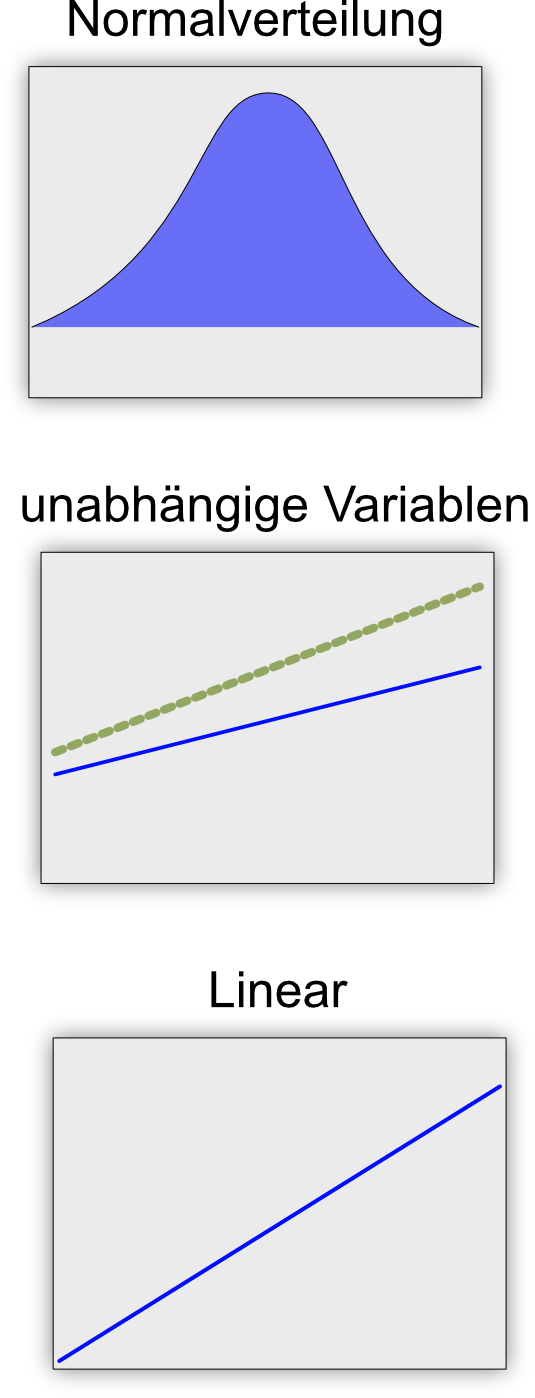
\includegraphics[width=0.6\linewidth]{Bilder/Regressions-Bedingungen.png}
 \captionof{figure}{Bedingungen lineare Regression}
\end{minipage}\hfill
\begin{minipage}[t]{0.45\linewidth}
\vspace{0pt}
Um die Lineare Regression erfolgreich anzuwenden müssen drei Bedingungen erfüllt sein:
\begin{itemize}
	\item Normalverteilte Daten
	\item Die Variablen sind unabhängig, d.h. die Werte beeinflussen sich nicht, im Gegensatz zum Beispiel bei Geschlecht und Schwangerschaft
	\item Die vorhergesagten Werte sind linear
\end{itemize}
Wenn diese Bedingungen nicht erfüllt sind kann die Lineare Regression kaum erfolgreich angewandt werden.
\end{minipage}
\end{center}

\subsection{GLM/GAM}
Lineare Regression hat einige Schwächen wie z. Bsp. die Annahme der Normalverteilung, nicht korrelierte Variablen oder auch einfach bei einem nichtlinearen Zusammenhang zwischen Eingang und dem Resultat. \acrfull{glm} und \acrfull{gam} erweitern Lineare Modelle um einen breiteren Anwendungsbereich zu ermöglichen.
\begin{center}
\begin{minipage}[t]{0.45\linewidth}
\vspace{0pt}
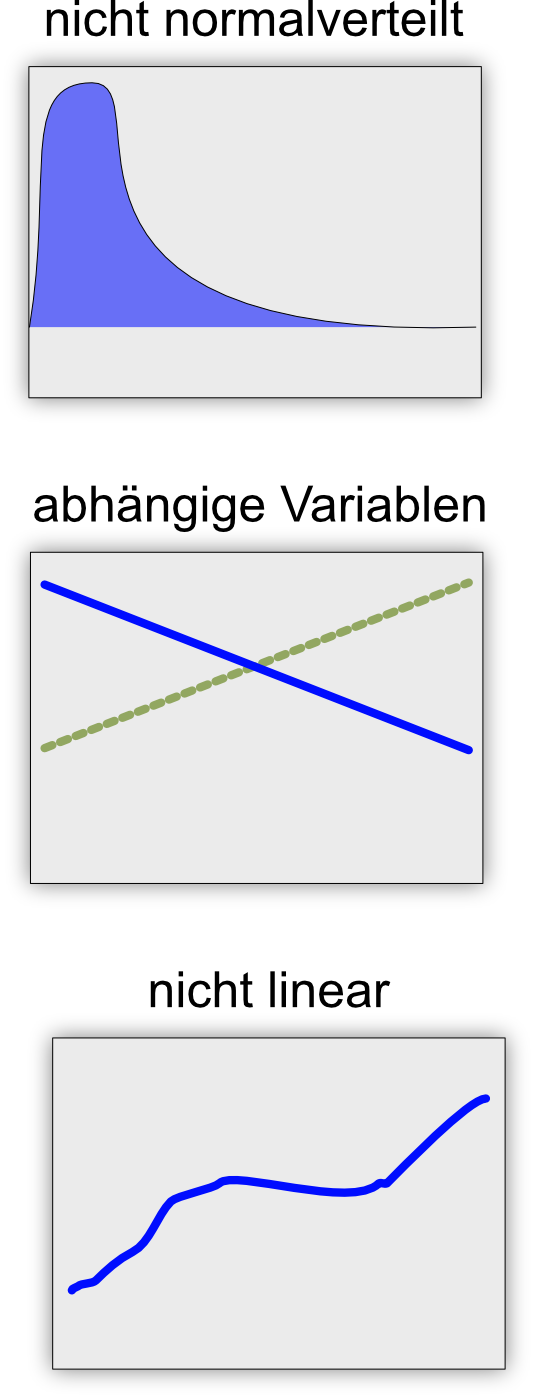
\includegraphics[width=0.6\linewidth]{Bilder/Regressions-Auschluss-Bedingungen.png}
 \captionof{figure}{Auschluss-Bedingungen lineare Regression}
\end{minipage}\hfill
\begin{minipage}[t]{0.45\linewidth}
\vspace{0pt}
Wenn die Voraussetzungen für eine Lineare Regression nicht erfüllt sind kann trotzdem mittels \Gls{glm} und \Gls{gam} eine Regression durchgeführt werden.
\end{minipage}
\end{center}

\subsection{Entscheidungsbäume}
Entscheidungsbäume (engl. Decision Tree) können bei einer geringen Anzahl von Parametern gut visualisiert werden.
\begin{center}
\begin{minipage}[t]{0.45\linewidth}
Die Regeln nach denen sich ein \Gls{DT} aufteilt können als Text dargestellt werden. Intuitiv besser verständlich sind jedoch grafische Darstellungen welche entweder den Baum als Struktur oder in einem Diagramm als Fläche darstellen.
\end{minipage}\hfill
\begin{minipage}[t]{0.45\linewidth}
\begin{lstlisting}
|--- petal width (cm) <= 0.80
|   |--- class: 0
|--- petal width (cm) >  0.80
|   |--- petal width (cm) <= 1.75
|   |   |--- class: 1
|   |--- petal width (cm) >  1.75
|   |   |--- class: 2
\end{lstlisting}
\end{minipage}
\end{center}

\begin{center}
\begin{minipage}[t]{0.45\linewidth}
\centering
	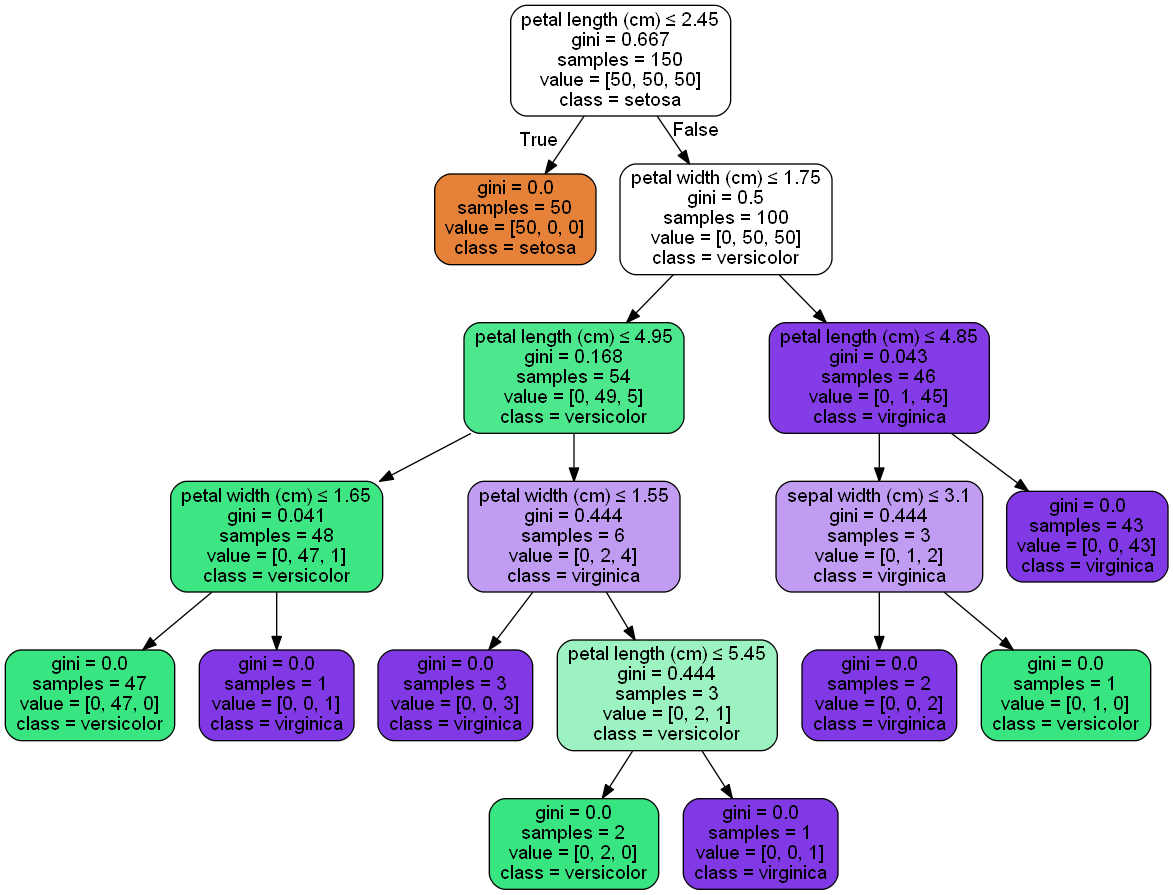
\includegraphics[width=\textwidth]{Bilder/iris-dt-explained.png}
	 \captionof{figure}{Entscheidungsbaum visualisiert.}
\end{minipage}\hfill
\begin{minipage}[t]{0.45\linewidth}
\centering
	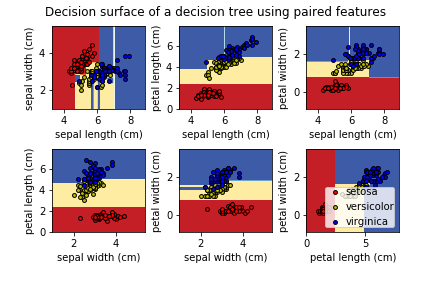
\includegraphics[width=\textwidth]{Bilder/iris-dt-decision-surface.png}
	 \captionof{figure}{Entscheidungsbaum als Flächen dargestellt}
\end{minipage}
\end{center}
Source Code \ref{dt-vis} (benötigt min. scikit-learn 0.22)

\subsection{RuleFit}
RuleFit \parencite{Friedman2008} verwendet Entscheidungsbäume um daraus Regeln abzuleiten welche neue Features erzeugen die von einem Linearen Modell verwendet werden. 
\subsection{Naive Bayes}

\section{Techniken für nicht direkt erklärbare Modelle}

\subsection{Grad CAM} \break
\Gls{GC} ist eine Technik \parencite{Selvaraju2016} um auf der Basis von Gradienten die für eine Bildklassifikation relevanten Bereiche eines Bildes hervorzuheben. Während die relevantesten Bereiche (gelb gefärbt) um den Kopf und vor allem den Ohren der Katze sind, zeigen die Darstellungen für die unpassenden Klassen auf Bereiche des Bodens.
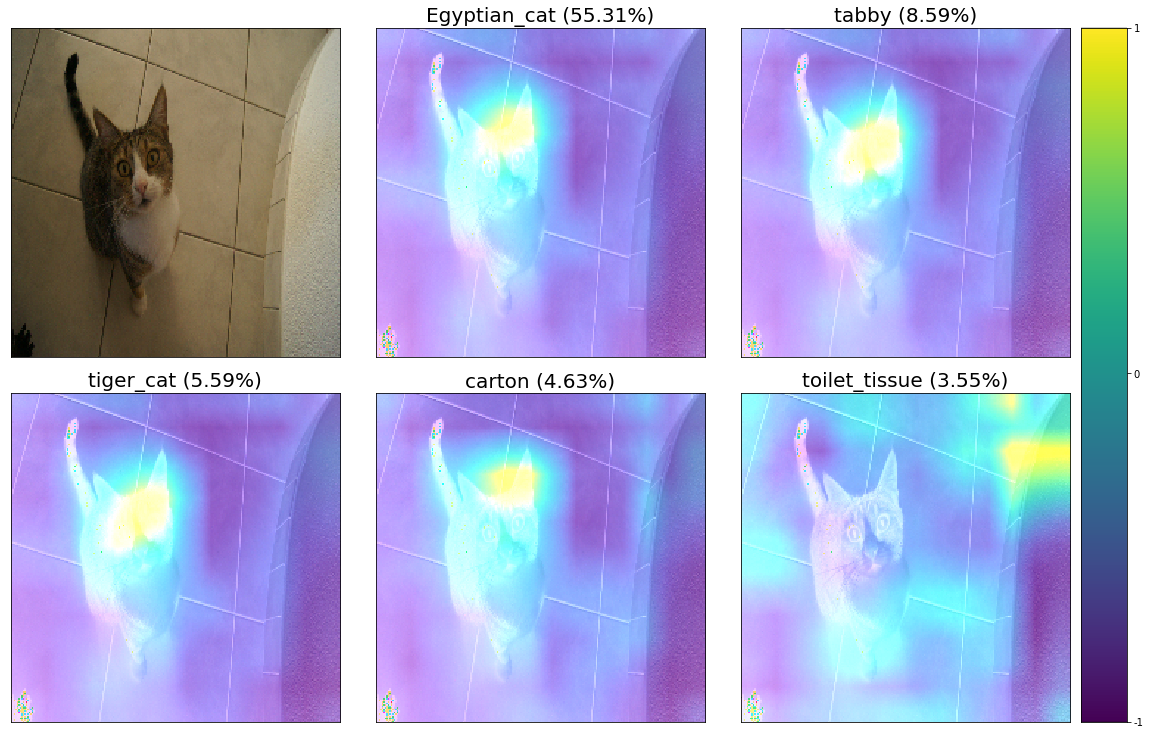
\includegraphics[width=\textwidth]{Bilder/Grad-Cam-Classes.png}

\subsection{Occlusion Sensitivity} \break
Eine weitere Variante um relevante Bildbereiche aufzudecken ist Occlusion Sensitivity. Mit diesem Verfahren tritt deutlicher als bei Grad CAM die Fokusierung auf den Boden bei den beiden Falschen Klassifizierungen zutage.
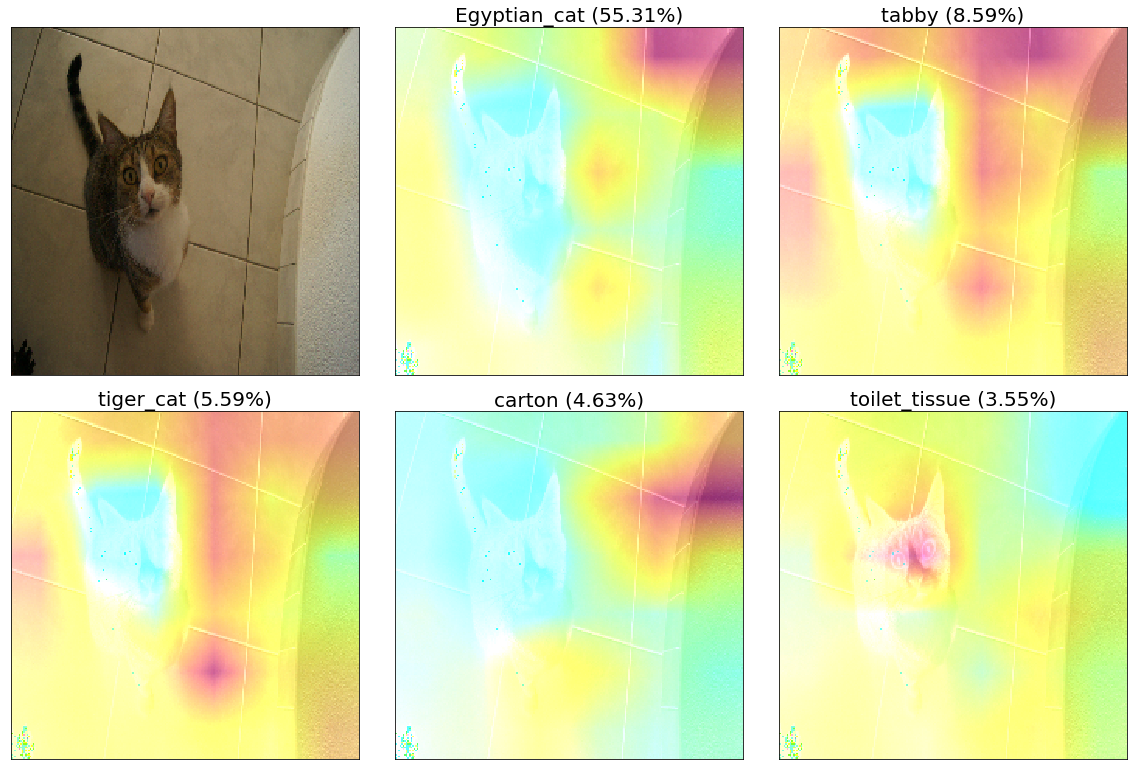
\includegraphics[width=\textwidth]{Bilder/OcclusionSensitivity-Classes.png}

\subsection{LRP}
\acrfull{lrp} ist eine Technik welche ebenfalls versucht die Vorhersage eines Klassifizierers zu erklären. 

\url{ttps://github.com/VigneshSrinivasan10/interprettensor}
\url{https://github.com/sebastian-lapuschkin/lrp_toolbox}

\subsection{Local Surrogate (LIME)}
\label{lime}
Die Technik LIME wurde 2016 erstmals vorgestellt \parencite{Ribeiro2016}. 
\Gls{lime} kann für verschiedene Arten von  \Gls{ML} Modellen, insbesondere auch Black Box Modelle, verwendet werden um eine Erklärung zu erzeugen. Dabei wird durch stetiges Verändern eines Eingangsbildes der Einfluss auf das Resultat geprüft. Mit den veränderten Eingangsdaten und den durch das Black Box Modell erzeugten Resultaten wird anschliessend ein neues Modell Trainiert das danach untersucht werden kann.

\paragraph*{}
Folgende Schritte werden bei der Anwendung von LIME durchgeführt:
\begin{itemize}
	\item Die Klasse für die man eine Erklärung erstellen will muss festgelegt werden
	\item Die ursprünglichen Daten werden verändert und die Resultate des Black Box Modells für diese Daten werden aufgezeichnet
	\item Die neu erzeugten Datensätzen werden nach der nähe zu der gesuchten Klasse gewichtet
	\item Ein neues Modell mit den gewichteten (neuen) Datensätzen wird erzeugt
	\item Die Vorhersage des Black Box Modells wird durch Interpretation des neu generierten Modelles erklärt
\end{itemize}
\break
In diesem Beispiel ist ersichtlich welche Bildbereiche (maskiert) nach \gls{lime} für das Resultat verantwortlich sind.

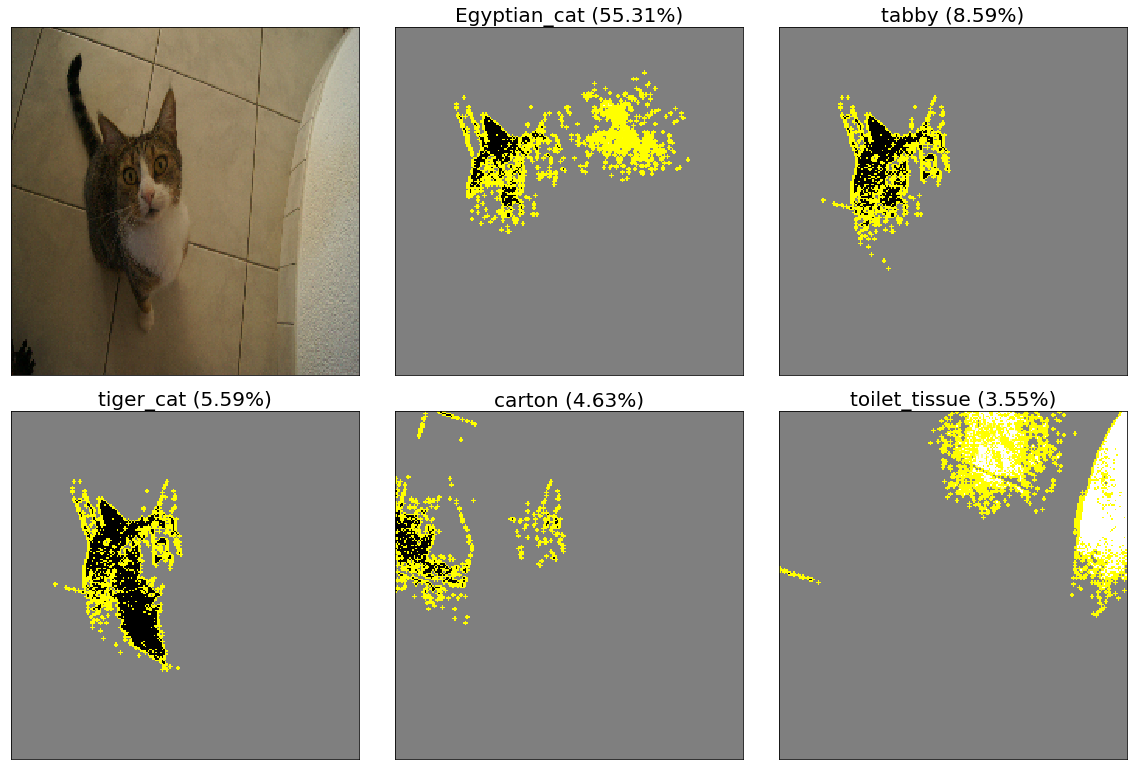
\includegraphics[width=\textwidth]{Bilder/Lime-Classes.png}
 \captionof{figure}{Darstellung relevanter Bildinhalte durch LIME}

Gegenüber den vorherigen Methoden ist LIME durch die Erzeugung temporärer Modelle bedeutend aufwendiger und dadurch auch langsamer.
\clearpage
\subsection{TCAV}
 \acrfull{tcav} wurde 2017 vorgestellt \parencite{Kim2017} und ist eine fortgeschrittene Methode um Erklärungen basierend auf den Bildinhalten zu generieren. Zu diesem Zweck werden zusätzliche Modelle als Beispiele für Bildinhalte erzeugt.
 
\break
 Ein als Zebra klassifiziertes Bild kann so zum Beispiel damit begründet werden dass auf dem Bild streifen und ein Pferd entdeckt wurden.
\begin{center}
\begin{minipage}[t]{\linewidth}
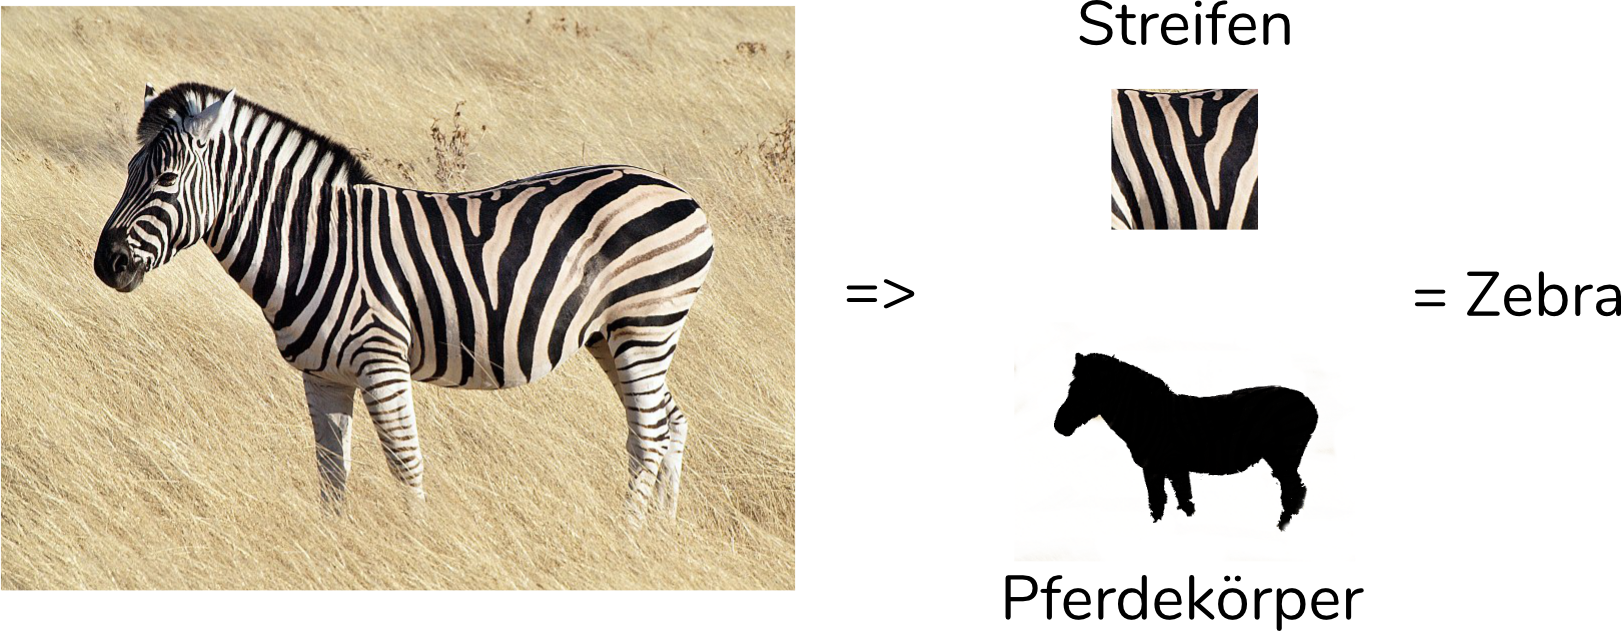
\includegraphics[width=\textwidth]{Bilder/Zebra-Explanation.PNG}
\caption{Darstellung Vorgehensweise TCAV}
\end{minipage}
\end{center}
Da bei diesem Verfahren für jede Kategorie von Bildbestandteilen ein Neuronales Netz trainiert werden muss, und für jedes Training Beispieldaten vorhanden sein müssen, ist der Aufwand gross. 

Eine Implementierung dieses Verfahrens kann unter folgendem Link auf Github gefunden werden: \cite{tcavLink}

\subsection{SVCCA}
\acrlong{svcca} \parencite{Raghu2017} vergleicht verschiedene Neuronale Netzwerke oder verschiedene Layer innerhalb des selben Neuronalen Netzwerkes.
\break
Durch den Vergleich der Vektoren verschiedener Klassen innerhalb des selben Netzes kann auf die Ähnlichkeit rückgeschlossen werden. Die beiden Klassen ``Husky'' und ``Eskimo Dog'' werden in der Untenstehenden Grafik als parallel verlaufende, beinahe überlappende Linien dargestellt, was auf die starke Ähnlichkeit der beiden Hunderassen hinweist.
\begin{center}
\begin{minipage}[t]{\linewidth}
 	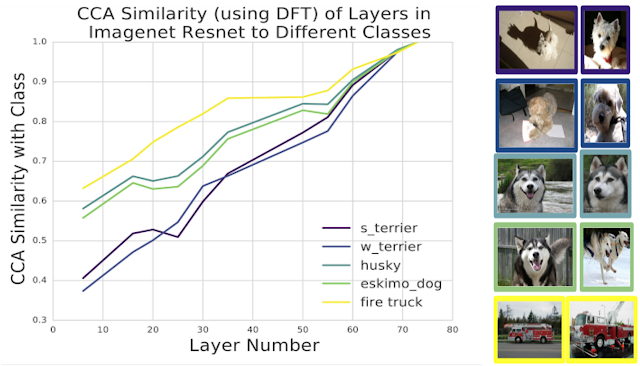
\includegraphics[width=\textwidth]{Bilder/svcca-similarities.png}
    	\caption{Vergleich Verschiedener Klassen mit SVCCA}
    	\caption*{Quelle: Google AI Blog, Interpreting Deep Neural Networks with SVCCA}
\end{minipage}
\end{center}
\cite{svccaLink}

\chapter{Konkrete Anwendung von XAI}

\section{Bilderkennung}
In den letzten Jahrzehnten wurden grosse Fortschritte in der Bilderkennung gemacht. Verantwortlich dafür sind vor allem Neuronale Netze, insbesondere die Techniken \acrfull{cnn} in Zusammenhang mit {dnn}. Neuronale Netze, insbesondere die für Bilderkennung weit verbreiteten \acrfull{dnn}, sind ohne weitere Hilfsmittel kaum zu analysieren.
Durch den starken Fokus auf Neuronale Netze bei der Bilderkennung sind für diese Technik auch einige Methoden vorhanden um das Verhalten eines Modelles  auf ein Bild darzustellen.
\subsection{WhiteBox Model: Klassifikation Hund - Katze}

\subsubsection*{Versuch: Eingangsdaten mit BIAS}
Daten welche für das trainieren von \Gls{ML} Modellen verwendet werden können eine unbekannt Struktur enthalten welche die gewünschte Vorhersage unrelevant ist, das Ergebnis jedoch verfälscht. Wenn ein solcher Effekt auftritt spricht man häufig von einem \Gls{KH}. Dieser Effekt trat bei einem Neuronalen Netz auf welches für einen Wettbewerb eingereicht wurde (Pascal VOC \cite{Everingham_thepascal}) und betraf die Erkennung von Pferden \parencite{Lapuschkin2019}. 

\begin{center}
\begin{minipage}[t]{0.45\linewidth}
\vspace{0pt}
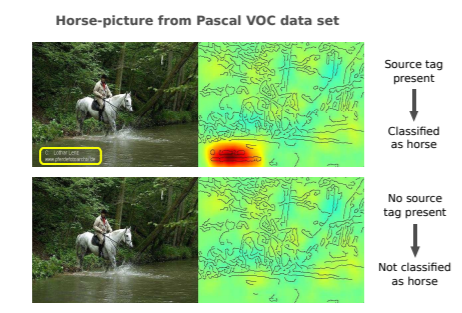
\includegraphics[width=\linewidth]{Bilder/HorsePredictionPascalVOC.PNG}
\caption{Klassifizierung eines Pferdes in Pascal VOC}
\caption*{Quelle: Unmasking Clever Hans Predictors and Assessing What Machines Really Learn \cite{Lapuschkin2019}}
\end{minipage}\hfill
\begin{minipage}[t]{0.45\linewidth}
\vspace{20pt}
Die meisten Bilder mit Pferden in dem bereitgestellten Trainingsdatensatz für die Pascal VOC Challenge enthielten einen Quellen Verweis. Aufgrund dessen lernte das Neuronale Netz anstatt des Erkennens von  Pferden, das Erkennen dieser Verweise. Da dieser Hinweis nur auf Pferdebildern vorhanden war wurden dadurch alle Bilder mit solch einem Hinweis als ``Pferd'' klassifiziert.
\end{minipage}
\end{center}

\break
In diesem Versuch soll diese Ausgangslage nachgestellt werden. Die Annahme ist dass ein grosser Teil der Bilder, welche Katzen darstellen, von einem Dienstleister stammen welcher sein Logo auf jedem Bild in der rechten unteren Ecke platzierte. 

\imgText{watermark.jpg}{fiktives Logo}{
 \vspace{20pt}
Um eine Verfälschung der Daten zu simulieren wurde nebenstehendes Logo in die Trainings- und Testdaten eingefügt. 
\break 
Insgesamt wurden 90\% der Katzenbilder mit diesem Logo gekennzeichnet. Hundebilder weisen kein Logo auf. \break Die Platzierung des Logos ist auf der linken Seite und, je nach Auflösung des Bildes, zwischen der unteren Ecke und der Mitte Bildes.
}

\begin{center}
\begin{minipage}[t]{0.45\linewidth}
	\centering
	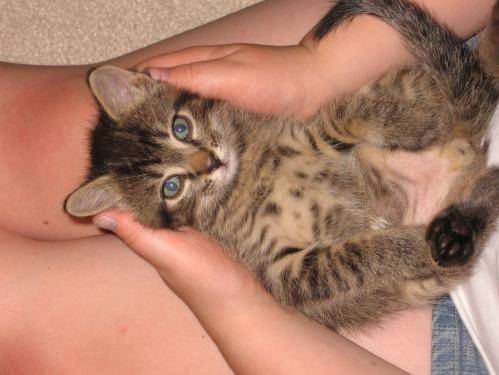
\includegraphics[width=\textwidth]{Bilder/cat_5.jpg}
	 \captionof{figure}{Ursprüngliches Bild}
\end{minipage}\hfill
\begin{minipage}[t]{0.45\linewidth}
	\centering
	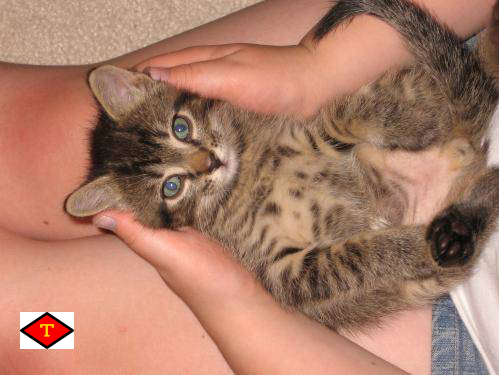
\includegraphics[width=\textwidth]{Bilder/cat_6.jpg}
	 \captionof{figure}{Manipuliertes Bild}
\end{minipage}
\end{center}

Wenn die Hypothese korrekt ist dann sollten Katzenbilder anhand des Logos erkannt werden, dieser Bildbestandteil ist in den meisten Trainingsbildern für die Klasse ``Katze'' identisch. Wenn nun ein Hundebild ohne Logo, welches korrekt als ``Hund'' klassifiziert wurde, noch einmal als geänderte Version mit Logo klassifiziert wird dann sollte die neue Vorhersage ``Katze'' lauten.

\subsubsection*{Aufbau des Neuronalen Netzes}
Die Grundlage bildet ein Blog Post in ``Towards Data Science''  \cite{dogVsCats}. Das erzeugte \acrshort{cnn} ist jedoch in der ursprünglichen Version ein \Gls{binClassificator}. Die für die Visualisierung gewählte Bibliothek ''tf\_explain'' \cite{tfExplain} kann jedoch keine binären Klassifizierer visualisieren weshalb das Model von mir auf die Erkennung von zwei Klassen angepasst wurde.

\begin{figure}
\begin{lstlisting}[language=Python]
model.add(Conv2D(32, 3, strides=(1, 1), padding='same', input_shape=input_shape, activation='relu'))
model.add(Conv2D(32, 3, strides=(1, 1), padding='same', activation='relu'))
model.add(MaxPooling2D(pool_size=(2, 2)))

model.add(Conv2D(64, 3, strides=(1, 1), padding='same', activation='relu'))
model.add(Conv2D(64, 3, strides=(1, 1), padding='same', activation='relu'))
model.add(MaxPooling2D(pool_size=(2, 2)))

model.add(Conv2D(128, 3, strides=(1, 1), padding='same', activation='relu'))
model.add(Conv2D(128, 3, strides=(1, 1), padding='same', activation='relu'))
model.add(MaxPooling2D(pool_size=(2, 2)))

model.add(Conv2D(256, 3, strides=(1, 1), padding='same', activation='relu'))
model.add(Conv2D(256, 3, strides=(1, 1), padding='same', activation='relu'))
model.add(MaxPooling2D(pool_size=(2, 2)))

model.add(Flatten())
model.add(Dense(256, activation='relu'))
model.add(Dropout(0.5))

model.add(Dense(256, activation='relu'))
model.add(Dropout(0.5))

model.add(Dense(2))
model.add(Activation('sigmoid'))
    
model.compile(loss='binary_crossentropy',
            optimizer=RMSprop(lr=0.0001),
            metrics=['accuracy'])
\end{lstlisting}
\end{figure}
\caption{CNN für Dog vs. Cats}

\subsubsection*{Training}
Über 20 Epochen wurde das \acrshort{cnn} trainiert, mit folgenden Resultaten:
\imgText{Training-Manipulated-LogLoss.png}{Log-loss / Accuracy Dog vs. Cat}{}

\imgText{Training-Manipulated-StatisticsTable.png}{Bewertung des Hund-Katze Netzwerkes}{

}

\subsubsection*{Hund ohne Logo}
\imgText{Manipulated_case_img7.png}{Testbild ohne Logo}{
Das Testbild eines Hundes wird von dem Netz eindeutig mit einer 99\% Wahrscheinlichkeit als Hund klassifiziert.
\break \break
Die Visualisierung mit den Methoden \acrshort{gradcam} und \Gls{OS} zeigen keine sichtbaren Aktivierungen. 
Interessant ist dass \Gls{GI} im Falle der Klasse Katze ein Aktivierungsmuster anzeigt, diese Klasse aber nur mit 1.18\% Wahrscheinlichkeit klassifiziert wird.
}

\subsubsection*{Hund mit Logo}
\imgText{Manipulated_case_img8.png}{Testbild mit Logo}{
Das gleiche Bild wird nun mit dem Logo versehen wie es auch auf den meisten Katzenbildern vorkommt. \break \break 
Die Klassifizierung ändert sich danach eindeutig: 100\% Katze. Das \Gls{NN} wurde konnte also dazu gebracht werden dem Logo die höchste Aufmerksamkeit zu widmen. 
\break \break
Dies kann durch die Visualisierung gezeigt werden. Während \Gls{GC} und \Gls{GI} kaum Aktivierungen aufzeigen, ist die Lage bei \Gls{OS} deutlich: Für die Klasse ``Katze'' spricht das Vorhandensein des Logos während für die Klasse ``Hund'' alle Bildbereiche ausser dem Logo relevant sind.
}

\subsubsection*{Katze ohne Logo}
\imgText{Manipulated_case_img4.png}{Testbild Katze ohne Logo}{
Dieses Bild einer Katze wurde zu 98.8\% als ``Hund'' klassifiziert. Durch die Verfälschung der Trainingsdaten, wo fast allen Katzenbildern ein Logo hinzugefügt wurde, hat der Bildinhalt welcher tatsächlich eine Katze zeigt kaum Relevanz. 
\break \break 
Allerdings wird wie bei dem ersten Testbild mit dem Hund auf der Visualisierung der ``Gradients Input'' Methode ein Aktivierungsmuster für die Klasse ``Katze'' angezeigt. Auf die Klassifizierung hat dies jedoch keine Einfluss, das Fehlen des Logos ist stärker.
}

\subsubsection*{Katze mit Logo}
\imgText{Manipulated_case_img5.png}{Testbild Katze mit Logo}{Wenn nun dem gleichen Bild mit der Katze das Logo hinzugefügt wird ist die Klassifizierung eindeutig: 100\% Katze
\break \break
Der Effekt des hinzugefügten Logos wird, wie schon bei dem Testbild mit dem Hund,  in der ``Occlusion Sensitivity'' Visualisierung eindrücklich dargestellt: Gegenüber dem Bildbereich mit dem Logo wird der Rest des Bildes ignoriert.
}

\subsubsection*{Testbilder ohne Katze oder Hund}
Da das \Gls{cnn} nur die beiden Klassen ``Katze'' oder ``Hund'' kennt muss jedes Bild, das als Input verwendet wird, einer der beiden Klassen zugeordnet werden. Eine Klasse ``Unbekannt'' oder ``Weder noch'' kann nicht vergeben werden. Trotzdem lassen sich durch die Verteilung der vorhergesagten Klassen Rückschlüsse ziehen.
\imgText{Manipulated_case_img1.png}{Testbild Sonnenblume}{
Obwohl auf diesem Bild keine Katze erkennbar ist wurde die Klassifizierung mit dem Ergebnis 100\% Katze eindeutig getroffen. Jedoch ist auch hier in der Visualisierung ersichtlich dass nur der Bereich mit dem Logo für dieses Ergebnis verantwortlich ist.
}
\imgText{Manipulated_case_img2.png}{Testbild Falter ohne Logo}{
Das Bild des Falters wird in seinem unverändertem Zustand sicher mit 99.9\% Wahrscheinlichkeit der Klasse Hund zugeordnet.
}
\imgText{Manipulated_case_img3.png}{Testbild Falter mit Logo}{
Wenn nun dem Ursprünglichen Bild noch das Logo hinzugefügt wurde dann wechselt die Vorhersage zu 100\% auf die andere Klasse ``Katze''.
}

\subsubsection*{Fazit dieses Versuches}
Durch die Verfälschung der Trainings- und Testdaten wurde aus einem ``Katze oder Hund'' Klassifikator eine Erkennung des Test-Logos erzeugt. In der Realität wären die unbrauchbaren Erkennungsraten schnell aufgefallen, durch die Visualisierungen mit \Gls{XAI} Techniken kann der Fehler aber eindeutig dem verfälschenden Bildelement zugeordnet werden.
\break 
Eine weitere Erkenntnis ist die dass von den drei verwendeten Visualisierungs-Methoden nur \Gls{OS} die Fokussierung auf das falsche Bildelement ersichtlich macht. 

\subsection{Vortrainiertes ImageNet Modell}
Das für die folgenden Analysen verwendete Modell stammt aus der ImageNet Challenge \parencite{imageNet} aus dem Jahr 2014 und ist frei verfügbar \parencite{Simonyan2014}. Ein ImageNet Model definiert 1001 Klassen von Objekten welche erkannt werden. Eine Klassifikation mit \parencite{TensorFlow} erzeugt eine Liste mit den Wahrscheinlichkeiten für alle Klassen. 

\subsubsection*{Versuch: Explorative Analyse der Bildklassifikation}
Mit den \gls{XAI} Techniken kann für jede Klasse visualisiert werden welche Bildbereiche für diese Klassifikation relevant sind. Mit diesem Versuch wurde versucht ein Verständnis über die Funktionsweise der Klassifizierung zu finden und bei fehlerhaften Klassifizierungen eine Erklärung für das falsche Resultat zu finden.

\subsubsection*{Test 1: Katzenbild}
Mittels dem Modell VGG16 aus der Tensorflow Bibliothek \textit{VGG16} \cite{vgg16} wurde folgendes Bild analysiert:
\imgText{Mira.jpg}{Original Testbild Katze}{
		
		\begin{tabular}{@{} *5l @{}}    \toprule
		\emph{Klasse} & \emph{Wahrscheinlichkeit} &&&  \\\midrule
		Egyptian cat & 55.31\% \\ 
		 tabby & 8.59\% \\ 
		 tiger cat & 5.59\% \\ 
		 carton & 4.63\% \\
		 toilet tissue & 3.55\% \\ \bottomrule
		 \hline
		\end{tabular}
}

Obwohl das vorhergehende Bild korrekt als Katze klassifiziert wurde (allerdings als die falsche Katzenrasse), fallen die 4. und 5. Klassifikation auf. Die Klassifizierung als Karton (4.6\%) oder Toilettenpapier (3.6\%) ist zwar nicht sehr wahrscheinlich, es stellt sich aber dennoch die Frage weshalb keine weiteren Tiere welche, optisch grössere Ähnlichkeit mit einer Katze aufweisen, gefunden wurden.

\subsubsection*{Test 2: Meerschweinchen, ähnlicher Hintergrund wie bei Bild mit der Katze}
Um festzustellen ob alleine der Bildhintergrund die (geringen) Wahrscheinlichkeiten für Toilettenpapier und Karton ausgelöst haben, wurde ein anderes Bild welches an der gleichen Stelle aufgenommen wurde, allerdings mit einem Meerschweinchen anstatt einer Katze, klassifiziert.
\imgText{IMG_2729.JPG}{Testbild Meerschweinchen}{

		\begin{tabular}{@{} *5l @{}}    \toprule
		\emph{Klasse} & \emph{Wahrscheinlichkeit} &&&  \\\midrule
		Cockroach & 31.89\% \\
		Australian terrier &  8.14\% \\
		English springer & 5.48\% \\
		Irish setter & 4.95\% \\
		Blenheim spaniel & 4.74\% \\
		Umbrella & 2.16\% \\
		Tick & 1.57\% \\
		Admiral & 1.53\% \\
		Weasel  & 1.34\% \\
		Centipede & 1.31\% \\
		Sussex spaniel & 1.00\% \\
		Irish water spaniel  & 0.99\% \\
		Papillon & 0.99\% \\
		Welsh springer spaniel  & 0.96\% \\
		Toilet tissue & 0.92\% \\ \bottomrule
		 \hline
		\end{tabular}
}
\break
Dieses Bild wurde falsch klassifiziert. Statt der korrekten Klasse ``Guinea Pig'' (Meerschweinchen) wurde die Klasse ``Cockroach'' (Kakerlake) gewählt. Allerdings ist die angegebene Wahrscheinlichkeit für ``Guinea Pig'' mit 32\% nicht sonderlich hoch. Das Toilettenpapier (``Toilet tissue''), welches im vorherigen Bild immerhin mit 3.6\% Wahrscheinlichkeit angegeben wurde, hat nun nur noch eine Wahrscheinlichkeit von 0.9\%.
\break
Anscheinend ist der Hintergrund in diesem Fall nicht alleine Ausschlaggebend für die Klasse Toilettenpapier. Mit den bereits vorgestellten Verfahren kann man nun die Einflüsse der einzelnen Bildpunkte auf die Klassifizierung sichtbar machen.

\subsubsection*{Analyse mittels Grad CAM}
\imgText{Oreo-Grad-Cam-Classes.png}{Testbild Meerschweinchen Grad CAM}{
Die erste Visualisierung zeigt den Einfluss der einzelnen Bildpunkte für die wahrscheinlichsten fünf Klassen mit dem Verfahren \Gls{GC}. Der Körper des Meerschweinchens ist in allen Fällen stark Relevant, wobei der helle Fleck am Hals des Tieres den grössten Einfluss auf die Klassifizierung hat. Der Hintergrund zeigt in fast allen Fällen einen Einfluss auf, insbesondere bei der Klassifikation ``Australian Terrier''.
}
Diese Analyse bringt keine Erklärung dafür weshalb eine Fehlklassifizierung statt gefunden hat, und auch die beiden eigenartigen Klassifizierungen des vorherigen Bildes sind nun nicht besser erklärbar. Aus diesem Grund wird nun die Analyse mit zusätzlichen Verfahren weitergeführt.

\subsubsection*{Analyse durch weitere Verfahren}
Um die Analyse des \Gls{cnn} durch visualisierende Verfahrend zu vereinheitlichen wurde ein Python Skript geschrieben welches die gewählten Visualisierungs-Verfahren abbildet und zusammen mit dem original Bild darstellt. Zusätzlich wird noch eine Tabelle dargestellt in welcher die fünf wahrscheinlichsten Klassen und, falls noch nicht bereits unter den ersten fünf, die korrekte Klasse für das Bild angezeigt werden.
\imgText{Oreo-Classification.png}{Testbild Meerschweinchen div. Verfahren}{
Die Visualisierungen für die Klassifizierung ``Cockroach''  zeigen kein einheitliches Muster: \break 
Während mittels \Gls{GC} vor allem der Körper des Meerschweinchens hervorgehoben wird, zeigt \Gls{GI} kaum Aktivität im Bereich des Meerschweinchens an. \break 
\Gls{OS} wiederum findet einen breiten Streifen welcher rechts und links über den Körper des Meerschweinchens hinausgeht als relevant und \Gls{limeG} markiert den Kopf des Tieres und einen schwach sichtbaren Fleck links daneben. \break
Die Visualisierung der eigentlich korrekten Klassifizierung ``Guinea Pig'' sieht auf den ersten Blick der Visualisierung von ``Cockroach'' ähnlich, es erstaunt aber dass die Methode \Gls{limeG} den Körper des Meerschweinchens fast vollständig hervorhebt, jedoch hat dies anscheinend keinen grossen Einfluss auf die Klassifizierung.
}

\subsubsection*{Analyse ursprüngliches Testbild durch weitere Verfahren}
\imgText{Mira-Classification.png}{Testbild Katze div. Verfahren}{
Mit der selben Technik wurde noch einmal das ursprüngliche Testbild analysiert.
}
\imgText{Mira-Classification-2-only-tabby.png}{}{}
\imgText{Merlin-Classification.png}{}{}
\imgText{Toilett-Tissue-Classification.png}{}{}


\section{Texterkennung}
Auch im Bereich der Texterkennung kann ein besseres Wissen über die Funktionsweise einer \Gls{MLg} Anwendung sowohl den Entwicklern als auch Anwendern helfen. Insbesondere bei den Problemstellungen Sentiment Analyse und Dokumenten Klassifikation kann \Gls{XAI} das Verständnis fördern.

\subsection{Stimmungs-Analyse von Film-Bewertungen}
Das folgende Beispiel visualisiert eine Sentiment Analyse von Bewertungen von Kinofilmen. Grundlage für das Experiment ist ein Tutorial \cite{movieReview} welches generell die Text Analyse mit \cite{scikit-learnLink} erläutert. Die Daten stammen aus einer Arbeit von Bo Pang and Lillian Lee \parencite{Pang+Lee2004} aus dem Jahre 2004 und sind ein Auszug von Film Reviews der Internetplattform IMDB. Jeweils 100 positive und negative Reviews werden, mit einem Testanteil von 20 Prozent, von einem RandomForest trainiert.

\parencite{textClassEli5}

\begin{lstlisting}[language=Python]
from sklearn.ensemble import RandomForestClassifier

classifier = RandomForestClassifier(n_estimators=1000, random_state=0)
classifier.fit(X_train, y_train)
\end{lstlisting}

\imgText{MovieReviews-SentimentClassification_ConfMatrix.PNG}{Konfusions-Matrix Texterkennungs-Experiment}{
}
Die Konfusionsmatrix mit einer für ein Experiment annehmbare Fehlerquote und einer Accuracy von 0.855.

\subsubsection*{Visualisierung durch ELI5}
Die Python Bibliothek \cite{ELI5} unterstützt einige \gls{ML} Bibliotheken und bietet die Möglichkeit Schlüsselwörter welche für eine Klassifikation relevant sind direkt in dem Ursprungstext darzustellen. 

\begin{center}
\begin{minipage}[t]{0.45\linewidth}
\vspace{0pt}
\centering
	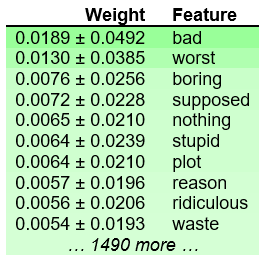
\includegraphics[width=0.7\textwidth]{Bilder/MovieReviews-SentimentClassification_Weights.PNG}
	 \captionof{figure}{Top Features Film Review Klassifizierung}
\end{minipage}\hfill
\begin{minipage}[t]{0.45\linewidth}
\vspace{20pt}
Eine Übersicht der Top Features zeigt die Funktion ``show\_weights()''.
\begin{lstlisting}[language=Python]
eli5.show_weights(classifier, vec=vectorizer, top=10)
\end{lstlisting}
Allerdings verhält sich ELI5 bei einer binären Klassifizierung so dass nur eine Klasse (in diesem Fall `neg') dargestellt wird. Die Farbe Grün stellt immer die aktuell gewählte Klasse dar weshalb hier auch negative Wörter grün eingefärbt sind.
\end{minipage}
\end{center}

Um einen Datensatz zu visualisieren verwendete man die Methode ``explain\_prediction()'', welche sowohl Details über die Features als auch eine Darstellung des Textes mit den hervorgehobenen Schlüsselwörtern anzeigt. Je nach verwendetem Modell weicht die Darstellung von dem hier dargestellten Bild ab, bei gewissen Tree Algorithmen (z.Bsp. DecisionTree) wird zusätzlich noch die Baumstruktur angezeigt.
\begin{lstlisting}[language=Python]
doc = documents[414]
eli5.explain_prediction(classifier, doc, vec=vectorizer,target_names=['neg','pos'], top=20)
\end{lstlisting}

\begin{center}
\begin{minipage}[t]{\linewidth}
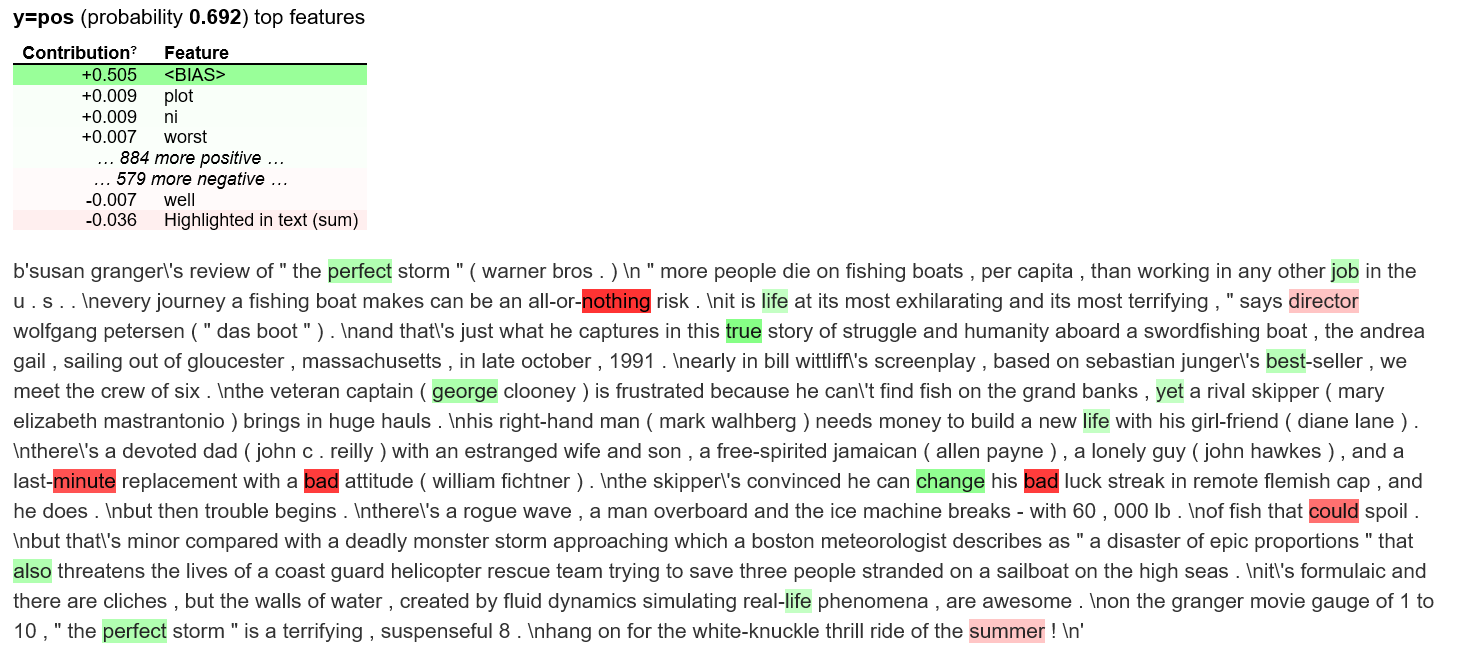
\includegraphics[width=\textwidth]{Bilder/MovieReviews-SentimentClassification_1.PNG}
\caption{Visualisierung positives Film Review}
\end{minipage}
\end{center}

Bei der Darstellung des negativen Film Reviews fällt auf dass Wörter welche für eine negative Stimmung stehen Grün markiert sind. Dies kommt daher dass für ELI5 die wahrscheinlichste Klasse `neg' ist (81\%) und deshalb alle Schlüsselwörter welche auf diese Klasse hinweisen grün markiert werden.

\begin{center}
\begin{minipage}[t]{\linewidth}
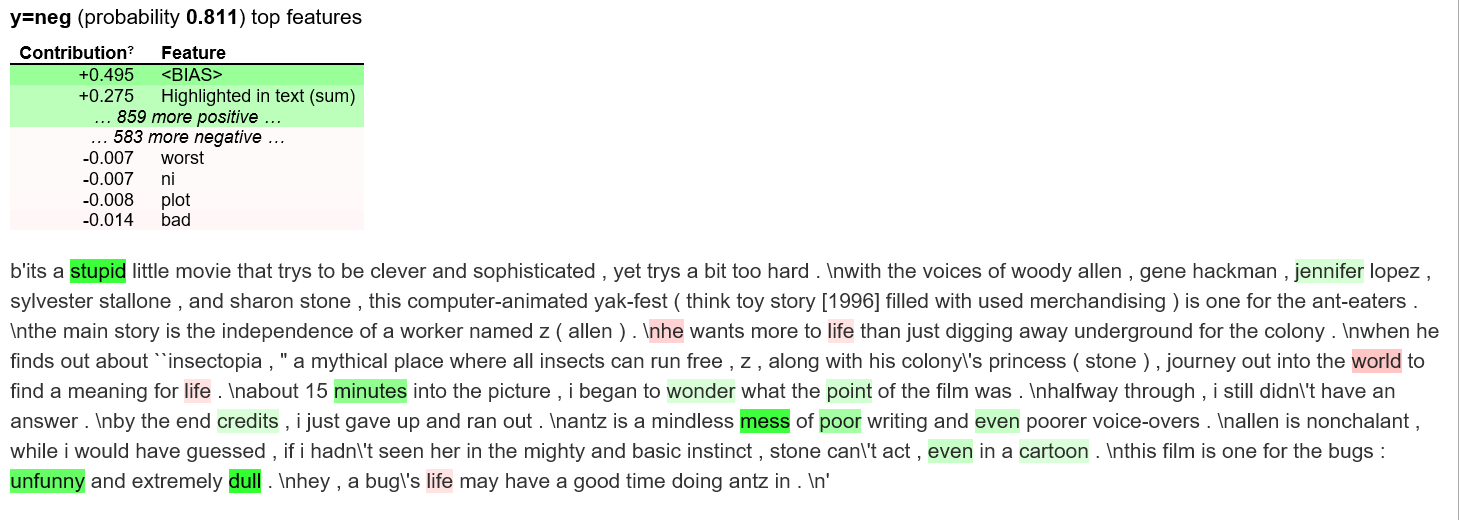
\includegraphics[width=\textwidth]{Bilder/MovieReviews-SentimentClassification_2.PNG}
\caption{Visualisierung negatives Film Review}
\end{minipage}
\end{center}

\subsubsection*{Blackbox Visualisierung mit ELI5}
Während in dem letzten Beispiel ein White Box Model angewendet wurde, kann \cite{ELI5} auch Black Box Modelle analysieren. Dazu verwendet \cite{ELI5} eine \Gls{lime} implementation und die Vorhersage zu erklären.

\chapter{Schwächen von ML Modellen erkennen}
\section{Diskriminierung durch Bias}
\section{Adversarial Attacks}
\section{Data Poisoning}

\chapter{Weiterentwicklung von XAI}

\chapter{Anhang}
\section{Source Code}
\label{dt-vis}

\subsection{Entscheidungsbaum Visualisierung mit sklearn und Graphviz}
\begin{lstlisting}[language=Python, caption=Decision Tree Visualisierung]
from sklearn.datasets import load_iris
from sklearn import tree
from sklearn import datasets

X, y = load_iris(return_X_y=True)
clf = tree.DecisionTreeClassifier()
clf = clf.fit(X, y)

iris = datasets.load_iris()

dot_data = tree.export_graphviz(clf, out_file=None, 
                      feature_names=iris.feature_names,  
                      class_names=iris.target_names,  
                      filled=True, rounded=True,  
                      special_characters=True)  

# print tree as text
from sklearn.tree import export_text
r = export_text(clf, feature_names=iris['feature_names'])
print(r)

# print tree as colored top-down tree
import graphviz
graph = graphviz.Source(dot_data)  
graph 

# plot decision surface
import numpy as np
import matplotlib.pyplot as plt
# Parameters
n_classes = 3
plot_colors = "ryb"
plot_step = 0.02

for pairidx, pair in enumerate([[0, 1], [0, 2], [0, 3],
                                [1, 2], [1, 3], [2, 3]]):
    # We only take the two corresponding features
    X = iris.data[:, pair]
    y = iris.target
    
    # Train
    dTree = tree.DecisionTreeClassifier().fit(X, y)

    # Plot the decision boundary
    plt.subplot(2, 3, pairidx + 1)

    x_min, x_max = X[:, 0].min() - 1, X[:, 0].max() + 1
    y_min, y_max = X[:, 1].min() - 1, X[:, 1].max() + 1
    xx, yy = np.meshgrid(np.arange(x_min, x_max, plot_step),
                         np.arange(y_min, y_max, plot_step))
    plt.tight_layout(h_pad=0.5, w_pad=0.5, pad=2.5)

    Z = dTree.predict(np.c_[xx.ravel(), yy.ravel()])
    Z = Z.reshape(xx.shape)
    cs = plt.contourf(xx, yy, Z, cmap=plt.cm.RdYlBu)

    plt.xlabel(iris.feature_names[pair[0]])
    plt.ylabel(iris.feature_names[pair[1]])

    # Plot the training points
    for i, color in zip(range(n_classes), plot_colors):
        idx = np.where(y == i)
        plt.scatter(X[idx, 0], X[idx, 1], c=color, label=iris.target_names[i],
                    cmap=plt.cm.RdYlBu, edgecolor='black', s=15)

plt.suptitle("Decision surface of a decision tree using paired features")
plt.legend(loc='lower right', borderpad=0, handletextpad=0)
plt.axis("tight")
\end{lstlisting}
https://scikit-learn.org/stable/modules/tree.html

\subsection{Bild-Klassifikation mit tf-explain}
Das folgende Programm erzeugt mit den Bibliotheken Tensorflow (2.0) und tf-explain und en Algorithmen ``Grad CAM'' und ``Integrated Gradients'' Visualisierungen einer Bild-Klassifizierung. 
\begin{lstlisting}[language=Python, caption=Visualisiertes Neuronales Netz mit Tensorflow und tf-explain]
import tensorflow as tf
from keras.applications.vgg16 import VGG16
from keras.preprocessing.image import load_img
from keras.preprocessing.image import img_to_array
from keras.applications.vgg16 import preprocess_input
from keras.applications.vgg16 import decode_predictions

model = tf.keras.applications.vgg16.VGG16(weights="imagenet", include_top=True)

#print(model.summary())

imageOrig = load_img('D:/Master Thesis/dogs-vs-cats/test/DSC05797.JPG', target_size=(224, 224))
imageArr = img_to_array(imageOrig)  #output Numpy-array

imageReshaped = imageArr.reshape((1, imageArr.shape[0], imageArr.shape[1], imageArr.shape[2]))

image = preprocess_input(imageReshaped)
predictions = model.predict(imageReshaped)

import numpy as np
top5predictions = np.argsort(predictions)[0,::-1][:5]

labels = decode_predictions(predictions)

for label in labels[0]:
    print('%s (%.2f%%)' % (label[1], label[2]*100))
    
from tf_explain.core.grad_cam import GradCAM
from mpl_toolkits.axes_grid1 import ImageGrid

def createImageGrid(imageOrig, predictions, labels, explainer, explainerArgs):
    camImages = [imageOrig]
    fig = plt.figure(figsize=(20., 20.))
    grid = ImageGrid(fig, 111,  # similar to subplot(111)
                 nrows_ncols=(2, 3),
                 axes_pad=0.5,  # pad between axes in inch.
                 )
    for class_index in top5predictions:
        camImages.append(explainer.explain(class_index=class_index, **explainerArgs))
    
    i = -1
    for ax, im in zip(grid, camImages):
        # Iterating over the grid returns the Axes.
        ax.set_xticks([])
        ax.set_yticks([])
        label = labels[0][i]
        if i >= 0:
            ax.set_title('%s (%.2f%%)' % (label[1], label[2]*100), fontsize=20)
        ax.imshow(im)
        i = i + 1

    plt.show()


explainer = GradCAM()
createImageGrid(imageOrig, predictions, labels, explainer, {'model': model, 'layer_name': 'block5_conv3', 'validation_data': data})

from tf_explain.core.gradients_inputs import GradientsInputs
explainer = GradientsInputs()
createImageGrid(imageOrig, predictions, labels, explainer, {'model': model, 'validation_data': (np.array([imageArr]), None)})

from tf_explain.core.integrated_gradients import IntegratedGradients

explainer = IntegratedGradients()
createImageGrid(imageOrig, predictions, labels, explainer, {'model': model, 'validation_data': (np.array([imageArr]), None)})
\end{lstlisting}
https://github.com/sicara/tf-explain

\subsection{Visualisierung einer Klassifikation mit lime}
Die Visualisierung mit lime benutzt als Grundlage das Tutorial ``Image Classification Kears'' \parencite{limeKeras}.
\begin{lstlisting}[language=Python, caption=Visualisiertes Neuronales Netz mit Tensorflow und lime]
import lime 
from lime import lime_image

explainer = lime_image.LimeImageExplainer()


explanation = explainer.explain_instance(np.vstack([imageArr]), model.predict, top_labels=5, hide_color=0, num_samples=1000)

from skimage.segmentation import mark_boundaries

camImages = [imageOrig]
fig = plt.figure(figsize=(20., 20.))
grid = ImageGrid(fig, 111,  # similar to subplot(111)
             nrows_ncols=(2, 3),
             axes_pad=0.5,  # pad between axes in inch.
             )
for class_index in range(0,5):
    temp, mask = explanation.get_image_and_mask(explanation.top_labels[class_index], positive_only=True, num_features=5, hide_rest=True)
    camImages.append(mark_boundaries(temp / 2 + 0.5, mask))

i = -1
for ax, im in zip(grid, camImages):
    # Iterating over the grid returns the Axes.
    ax.set_xticks([])
    ax.set_yticks([])
    label = labels[0][i]
    if i >= 0:
        ax.set_title('%s (%.2f%%)' % (label[1], label[2]*100))
    ax.imshow(im)
    i = i + 1

plt.show()
\end{lstlisting}

\appendix
% Glossary
\printglossary[type=\acronymtype]
\printglossary[type=main]
% List of Figures
\listoffigures
% List of Tables
\begingroup
\let\clearpage\relax
\listoftables
% Bibliography
\printbibliography[type=article,title={Literaturverzeichnis Artikel}]

\printbibliography[type=book,title={Literaturverzeichnis Bücher}]

\printbibliography[type=misc,title={Linkverzeichnis}]
%Index
\addcontentsline{toc}{chapter}{Index}
%\printindex
% Appendices
\lstlistoflistings
\endgroup

\end{document}
